% Page: Random intercepts
% sources/book/chapters/08-random-intercepts.qmd
% One covariate, so the page's mean beta_0 + X^T beta is the line
% beta_0 + beta_1 x. Each block adds its own alpha_j and the points
% scatter by epsilon. The three lines are parallel, so the within-block
% correlation is positive: sigma_A^2 / (sigma_A^2 + sigma^2).
% Schematic points, not a recorded sample.
\documentclass[border=6pt]{standalone}
\usepackage[T1]{fontenc}
\usepackage{lmodern}
\usepackage{amsmath,amssymb}
\usepackage{tikz}
\usetikzlibrary{arrows.meta}
\usepackage{pgfplots}
\pgfplotsset{compat=1.18}
\definecolor{ink}{HTML}{1F2430}
\definecolor{statblue}{HTML}{174A7E}
\definecolor{grey}{HTML}{5E6A75}
\pgfplotsset{
  stat/.style={
    scale only axis,
    axis lines=left,
    axis line style={ink, line width=0.6pt},
    tick style={ink, line width=0.45pt},
    tick label style={font=\small, text=ink},
    label style={font=\small, text=ink},
    title style={font=\small, text=ink, align=center},
    unbounded coords=jump,
    scaled ticks=false,
    clip=false,
  },
}
\begin{document}
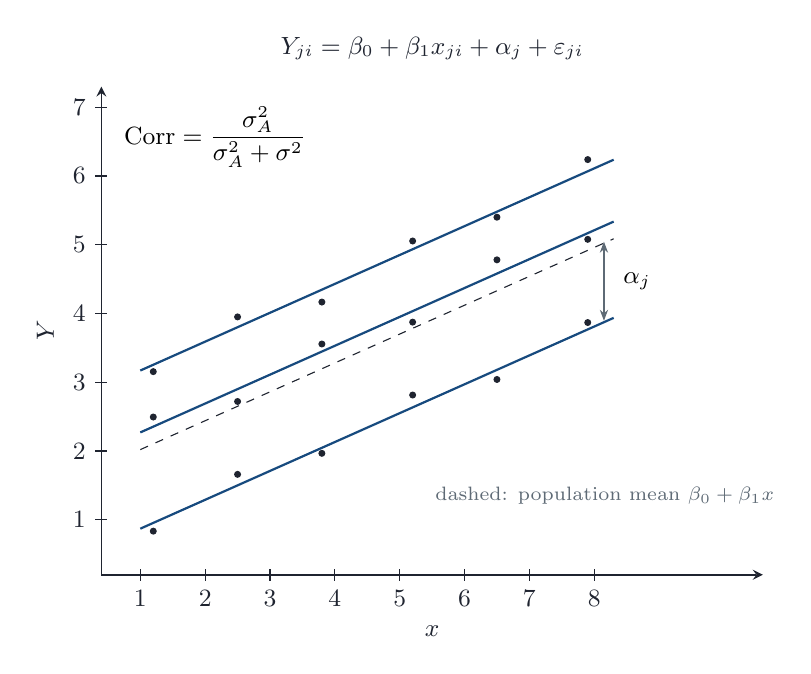
\begin{tikzpicture}
\begin{axis}[
  stat, width=8.4cm, height=6.2cm,
  xmin=0.4, xmax=10.6, ymin=0.2, ymax=7.3,
  xtick={1,2,3,4,5,6,7,8},
  ytick={1,2,3,4,5,6,7},
  xlabel={$x$},
  ylabel={$Y$},
  title={$Y_{ji}=\beta_0+\beta_1 x_{ji}+\alpha_j+\varepsilon_{ji}$},
]
  \addplot[ink, dashed, thin, domain=1:8.3, samples=2, forget plot] {1.6+0.42*x};
  \addplot[statblue, line width=0.8pt, domain=1:8.3, samples=2, forget plot] {1.6+0.42*x-1.15};
  \addplot[statblue, line width=0.8pt, domain=1:8.3, samples=2, forget plot] {1.6+0.42*x+0.25};
  \addplot[statblue, line width=0.8pt, domain=1:8.3, samples=2, forget plot] {1.6+0.42*x+1.15};
  \addplot[only marks, mark=*, mark size=1.05pt, ink, forget plot] coordinates {
    (1.2,0.834) (2.5,1.660) (3.8,1.966) (5.2,2.814) (6.5,3.040) (7.9,3.868)
    (1.2,2.494) (2.5,2.720) (3.8,3.556) (5.2,3.874) (6.5,4.780) (7.9,5.078)
    (1.2,3.154) (2.5,3.950) (3.8,4.166) (5.2,5.054) (6.5,5.400) (7.9,6.238)
  };
  \draw[{Stealth[length=1.4mm]}-{Stealth[length=1.4mm]}, grey, thin]
    (axis cs:8.15,3.894) -- (axis cs:8.15,5.044);
  \node[font=\small, anchor=west] at (axis cs:8.30,4.47) {$\alpha_j$};
  \node[font=\scriptsize, grey, anchor=west] at (axis cs:5.4,1.35)
    {dashed: population mean $\beta_0+\beta_1 x$};
  \node[font=\small, anchor=north west, align=left] at (axis cs:0.6,7.15) {%
    $\displaystyle\operatorname{Corr}=\frac{\sigma_A^{2}}{\sigma_A^{2}+\sigma^{2}}$};
\end{axis}
\end{tikzpicture}
\end{document}
